% \documentclass{article}
% \usepackage[utf8]{inputenc}
% \usepackage{amsmath}
% \usepackage{natbib}
% \usepackage{graphicx}
% \usepackage{astrojournals} % Necesario para nombres de revistas en luis-ref.bib
% \usepackage[spanish, es-minimal]{babel}
% \bibliographystyle{apj}


% \title{Catalog of stationary bowshock arcs in the Orion Nebula}

% \begin{document}
% \maketitle

% \section{Observaciones y descricción de los datos }

\label{chap:theori}

Este capítulo los hemos divido en dos partes. La primera parte es una descripción de la derivación de los parámetros físicos que gobiernan la naturaleza y estructura de los choques de proa, a partir de las suposiciónes; de que los arcos hiperbólicos y los choques de proa de los proplyds son estacionarios, como una posible consecuencia del equilibrio de presiones; que la cáscara chocada está dominada por la presión térmica y que el flujo de partículas  interno y externo que interaccionan para formar los arcos, están dominados por las presiones hidrodinámicas. Se ilustra que en la cáscara chocada se usó la ecuación de estado de los gases ideales para estimar la presión en esta región, como esta relación está en función de la densidad numérica de partículas, entonces antes de esto construimos una ecuación de la densidad promedio de partículas en función de los parámetros observacionales ya conocidos, esto es en términos del brillo superficial de \ha{} (\(S_{\ha{}}\)), el radio de curvatura (\(R_{c}\)) y el espesor (\(h\)) de la cáscara chocada. En las regiones externas e internas al choque se usó la presión ram y la ecuación general de la tasa de pérdida de masa para escribir las  presiones de los vientos internos y externos al choque en términos de la tasa de perdida de masa (\(\dot{M}\)), la velocidad del viento \(v\) y las distancias caracteristica (\(D\) y \(R_{0}\)), permitiendonos al mismo tiempo usando el equilibrio de presiones escribir el producto \(\dot{M}_{w}V_{w}\) del viento externo en términos de la presión térmica.\\

La segunda parte de este capítulo es una descripción de los resultados astrofísicos. Se muestran los resultados de las estimaciones realizadas de la densidad en la cáscara chocada, la presion en la cáscara, la presion de los vientos involucrados en los choques y el flujo momento interno de los objetos de nuestro catálogo, usando los ecuaciones derivadas en la primera parte del capítulo, junto con los parámetros observacionales medidos previamente directo de las observaciones, nos referimos aqui, al brillo superficial de \ha{}  \(S(\ha{})\), los radios de curvatura \(R_{c}\), la distancia de la estrella central al choque a lo largo del eje del arco \(R_{0}\) y la anchura de la cáscara \(h\), puesto que estos parámetros son variables de las ecuaciones derivadas teóricamente.

\section{Derivación de los parámetros físicos}
\label{sec:phy}

\subsection{Densidad  en la cáscara chocada }
\label{sec:densinty}

Un parámetro físico importante para estudiar la naturaleza de los choques de proa, es la densidad electrónica, así que un primer paso en esta tarea consiste en determinar la densidad promedio de partículas en la cáscara chocada. No obstante existen dos técnicas para estimar esta cantidad física. Una primera técnica consiste en medir la densidad promedio de electrones a través de las observaciones de los efectos de la desexcitación colisional. Esto puede hacerse comparando las intensidades de dos líneas emitidas por un mismo ión desde niveles con energía de excitación similares, así que las tasas de excitación relativas de los dos niveles dependen únicamente del cociente de sus fuerzas de colisión. Si los niveles tienen diferentes probabilidades de transición o diferentes tasas de desexcitación colisional, entonces la población relativa de los dos niveles dpenderá de la densidad, y por consiguiente el cociente de las intensidades de las líneas emitidas también dependerán de la densidad. Los mejores ejemplos de cociente de líneas usados para determinar la densidad electrónica en el rango del óptico son \(\oii~\lambda 3729/\lambda 3726\) y \(\sii~\lambda 6716/\lambda 6731\) \citep{Osterbrock:1989}.\\

La segunda técnica para estimar la densidad electrónica promedio en la cáscara de los choques de proa consiste en usar el brillo superficial de \ha{}, \(S(\ha{})\), obtenido a partir de las observaciones (más adelante daremos más detalles de este método). \citet{Henney:2013a} estimó la densidad electrónica para la cáscara de LL1, usando los dos métodos, es decir empleó el conciente de líneas de \sii{}~\(\lambda 6716/\lambda 6731\) para calcular la densidad en esta zona , y separadamente usó el brillo superficial de \ha{} para el mismo fin, posteriormente comparando los dos resultados encontró que las densidades derivada a partir de los dos métodos fueron muy compatibles. Por tanto para este trabajo hemos utilizado la segunda técnica para estimar la densidad, puesto que contamos con el brillo superficial de \ha{} de la cáscara de todos los arcos de proa de nuestro catálogo, entonces a continuación presentamos una análisis detallado de como determinar la densidad electrónica a partir del brillo superficial de \ha{}, pero antes es importante a hablar un poco sobre la naturaleza de la línea de recombinación de Balmer-\ha{}, debido a que a partir de la emisión de esta línea de recombinación medimos \(S(\ha{})\).    

\subsubsection{Líneas de recombinación de \ha{}}
\label{sec:lines-ha}

La serie de Balmer es un conjunto de líneas espectrales del átomo de hidrógeno que a diferencia de otras líneas de emisión del mismo, las transiciónes ocurren desde los niveles de energía \(n= 3,4,5,...\) al nivel \(n=2\) con \(n\) el número cuántico principal, así cada una de estas transiciones corresponde a una longitud de onda partícular (\(\lambda_{32}\) = 6563~\A~(\ha{}; rojo), \(\lambda_{42} = 4862~\A{}\) (\(\mathrm{H}\beta\); turquesa), \(\lambda_{52} = 4340~\A{}\) (\(\mathrm{H}\gamma\); azul) y \(\lambda_{62} = 4101.75~\A{}\) (\(\mathrm{H}\delta\); violeta)) estas longitudes de onda se han determinado a partir de datos experimentales, además éstas longitudes de onda \(\lambda\) caen dentro de la región visible del espectro electromagnético \citep{Carroll:1996}) (ver figura ). Por otro lado, para las líneas de recombinación del átomo de hidrógeno tenemos que la energía de los fotones que se emiten durante las transiciónes está dada por,

\begin{equation}
  \label{eq:energy}
  E = \frac{hc}{\lambda}. 
\end{equation}
 
Según el tratado de Bohr la energía en un estado cuántico es

\begin{equation}
  \label{eq:quantum}
  E_{n} = -13.6~\text{eV}~\frac{1}{n^{2}},
\end{equation}

esta última expresión también nos proporciona la energía del fotón emitido, es decir

\begin{equation}
  \label{eq:energy-}
 E = 13.6~\text{eV}~\left(\frac{1}{n_{\text{Inf}}^{2}}-\frac{1}{n_{\text{Sup}}^{2}}\right).
\end{equation}

 Donde esta es la energía liberada cuando el electrón decae de un nivel de energía, \(n_{\text{Sup}}\), a un nivel de menor energía, \(n_{\text{Inf}}\). Usando las ecuaciones~\ref{eq:energy} y \ref{eq:energy-} para el caso particular de las líneas de recombinación de \ha{} (donde la transición ocurre del nivel superior de energía \(n=3\) al nivel inferior de energía \(n=2\)) tendremos que: 

\begin{equation}
 \label{eq:values-energy-landa}
  E_{32} = 1.889~\text{eV}  ~~ \text{y} ~~
  \lambda_{32} = 6563~\A{}.
 \end{equation}

\subsubsection{Estimación de la densidad a partir del brillo superfical de \ha{} }
\label{sec:brillo}

Empezemos por escribir la relación de brillo superficial, suponiendo que no hay abosorción y que además está corregida por la absorción del polvo;

\begin{equation}
  \label{eq:brillo}
  S_{\ha{}} = \int \eta_{\ha{}} d\zeta \simeq \eta_{\ha{}} \Delta \zeta
\end{equation}  

\noindent en la que  \(\eta_{\ha{}}\) es la emisividad, cuyas unidades son [\(\mathrm{erg~s^{-1}~cm^{-3}~sr^{-1}}\)] y \(\Delta \zeta\) es el camino de la línea de visión a través de la cáscara (más adelante determinaremos \(\Delta \zeta\)). El primero de estos parámetro está dado por,

  \begin{equation}
    \label{eq:emision-coeficiente}
    \eta_{\ha} = \frac{N(\text{H}^0_{n=3})A_{32}}{4 \pi} \left(\frac{hc}{\lambda_{32}}\right) 
  \end{equation}

donde \(A_{32}\) es la probabilidad de transición y \(N(\text{H}^0_{n=3})\) es la densidad numérica de átomos neutros. Si la tasa de recombinaciones por volumen que producen \ha{} es 
\begin{equation}
  \label{eq:recombinaciones}
  \alpha_{\ha} N_{e}N_{H}=N(\text{H}^0_{n=3})A_{32}
\end{equation}

donde  \(\alpha_{\ha}\), \(N_{e}\) y \(N_{\text{H}}\)  son el coeficiente de recombinación efectiva, la densidad de electrones y la densidad de núcleos de hidrógeno. El coeficiente de recombinación efectiva  expresa la probabilidad de que un electrón en el estado \(n=3\) decaiga en cascada hasta el nivel de menor energía \(n=2\), considerando todos los caminos posibles, el cual está definido por 

\begin{equation*}
  \label{eq:coef}
  N_{\text{H}}N_{e}\alpha_{\ha} = \frac{4\pi j_{\ha}}{h\nu_{\ha}}
\end{equation*}

donde \(h\nu_{\ha}\) representa la diferencia de energía entre los niveles involucrados en la transición y \(j_{\ha}\) es la intensidad media de la línea de \ha{}. Según \citet{Osterbrock:2006} el coeficiente de recombinacíon efectiva de \ha{} tiene por valor  \(\alpha_{\ha}=1.27\times 10^{-13}\cm^{3}~\text{s}^{-1} \) para una temperatura electrónica de \(T=9000~\K\).\\


Por otro lado, al sustituir la Ec. \ref{eq:recombinaciones} en la Ec.~\ref{eq:emision-coeficiente} y teniendo en cuenta que \(N_{e}\simeq N_{\text{H}} \simeq N\) obtenemos que

\begin{equation}
 \eta_{\ha} =  \frac{\alpha_{\ha}N^{2}}{4\pi} \left(\frac{hc}{\lambda_{32}}\right)  
\end{equation}

 usando la ec. (\ref{eq:brillo}) se concluye que,

\begin{equation}
  \label{eq:densidad}
  N^{2}=\frac{4 \pi S_{\ha}}{\alpha_{\ha} E_{32} \Delta \zeta}
\end{equation}

\noindent esta expresión representa la densidad promedio en la cáscara, donde \( E_{32} = hc/\lambda_{32}\) es la energía de los fotones de \ha{} y cuyo valor es perceptible en la expresión~\ref{eq:values-energy-landa}. 


\subsubsection{Proyección en el plano del cielo}
\label{sec:pro}

Otra cosa que debemos  tener en cuenta en relación a los distancias y radios medidios a partir de las observaciones es que vemos a los choques de proa proyectados en el plano del cielo (\(x, y\)), entonces tendremos que las distancias (\(D\)), y los  radios caracterísiticos (\(R_{0}\) y \(R_{c}\)) medidos en la sección anterior no son estimaciones reales de los mismos, puesto que hay que considerar una rotación de los choques con respecto a \thC{}. Esto implica que las distancias y radios reales están rotados un ángulo \(i\) con respecto al marco de referencia del observador (\(x, y, z\)), en este orden de ideas los parámetros observacionales proyectados descritos anteriormente están dados por,

\begin{equation*}
  R_{c} = R'_{c};~~
  D = D' \cos i;~~ 
  R_{0} = R'_{0} \cos i
\end{equation*}

Donde los parámetros primados se ubican en el marco de referencia del objeto en cuestión (\(x', y', z'\)), es decir son las distancias y radios reales. La relación entre el radio curvatura proyectado y real permanece constante por que en este caso se considera una aproximación esférica donde el radio de curvauta no varía con el marco de referencia. 

\subsubsection{Estimación de la longitud del camino de la línea de visión, \(\Delta \zeta\)}
\label{sec:camino}

\begin{figure}
  \centering
  \includegraphics[width=.8\linewidth, clip]{figuras-tesis/geometry-chock.jpg}
  \caption{Geometría de la cáscara chocada. En el que se supone simetría cilíndrica en el plano del cielo (\(x, y\)), la línea de visión va en dirección al eje de las \(z\).}
  \label{fig:geometria}
\end{figure}

Para una cáscara localmente esférica con radio de curvatura \(R_{c}\) y anchura \(h\) que es observado tangencialmente \citeauthor{Henney:2013a}, suponiendo simetría cilíndrica y el eje de simetría en el plano del cielo (\(x, y\))(ver figura~\ref{fig:geometria1})  \ref{fig:geometria}), la longitud máxima de la línea de visión es


\begin{equation}
  \label{eq:line-singht}
   \Delta \zeta = 2\sqrt{2R_{c}h -h^{2}}
\end{equation}

 esto es considerando que la geometría de la cáscara en (\(x, z\)) es igual en (\(x, y\)) (ver figura  \ref{fig:geometria}). Para el caso en que \(h \gg R_{c}\) tendremos que,

\begin{equation}
  \label{eq:vision}
  \Delta \zeta = 2(R_{c}h)^{1/2}
\end{equation}

\begin{figure}
  \centering
  \includegraphics[width=.8\linewidth, clip]{figuras-tesis/geometry-shock2.jpg}
  \caption{Geometría de la cáscara en el plano (\(x, z\)), donde su radio de curvatura \(R_{c}\) es igual que en el plano (\(x, y\)).}
  \label{fig:geometria1}
\end{figure}

\subsection{Presión Térmica en la cáscara chocada}
\label{sec:pressur-thermal}

En la cáscara chocada la presión dominante es la presión térmica, debido a que esta zona esta contituida por gas ionizado, esto porque la energía cinética del flujo de partículas cargadas proveniente de la estrella central o proplyd se convierte en energía térmica en la zona chocada, entonces en este sentido tendremos que,

\begin{equation}
  \label{eq:presion-cascara}
  P_{\text{Termica}} = 2 N k T 
\end{equation}
 
Donde \(N\) dada por la Ec. \ref{eq:densidad} es la densidad total de partículas, \(k\) la constante de Boltzmann y \(T\) la temperatura en la cáscara chocada. Vamos a considerar que el gas en la zona chocada de los arcos de emisión están en equilibrio de fotoionización a una temperatura  de  \(\simeq10^{4}~\K\) \citep{Henney:2002, Henney:2002a}. No obstante, como se dijo en el capítulo~\ref{chap:introduction} inmediatamente detrás de cada uno de los choques que limitan la cáscara chocada la temperatura del gas se elevará por la termalización de la energía cinética pre-choque, pero este exceso de energía termal es radiada resultando en  una gran emisión y de esta manera el gas retorna a su estado de equilibrio, esto quiere decir que las longitudes de enfriamiento en la cáscara es mucho menor que la anchura de la zona chocada (\(d_{\text{cool}} \ll h\)), lo que indica que el  enfriamiento es bastante  eficiente y por tanto el gas en esta zona alcanza un equilibrio térmico a una temperatura de  \(\simeq10^{4}~\K\). Para este caso también hay que considerar la suposición de que los campos magnéticos no son importantes.\\

Por otro lado, si se incluye la contribución de helio entonces la densidad total de partículas es,

\begin{equation*}
  \label{eq:particulas}
  N = N_{\text{H}} + N_{e} + N_{\text{He}} + N_{z}
\end{equation*}

donde \(N_{e}\) es la densidad numérica de electrones, \(N_{\text{He}}\) es la densidad numérica de átomos de helio y \(N_{z}\) es la densidad de los elementos más pesados, esta última se puede despreciar debido a que su abundancia es pequeña. Es de notar que la abundancia por número de helio es \(y_{\text{He}}\) de tal manera que, \(N_{\text{He}} = y_{\text{He}} N\) con \(y_{\text{He}} \simeq 0.08\). Ahora podemos escribir la densidad electrónica como;

\begin{equation*}
  \label{eq:densidad-electronica}
  N_{e}=Nx_{\text{H}^{+}} + y_{\text{He}}Nx_{\text{He}^{+}} + 2 y_{\text{He}}Nx_{\text{He}^{++}} + \sum_{k} \sum_{j}Njy_{j}x_{jk}
\end{equation*}

Aquí \(x_{\text{H}^{+}}\) y \(x_{\text{He}^{+}}\) representan el grado de ionización del hidrógeno y el helio respectivamente, donde \(x_{\text{H}^{+}}=1\) y \(x_{\text{He}^{++}} \simeq 0\) para Orión, el último término de la expresión anterior es despreciable debido a que corresponde a los metales, de este modo nos queda

\begin{equation*}
  \label{eq:density}
  N_{e} \simeq N(1 +  y_{\text{He}}x_{\text{He}^{+}})
\end{equation*}

 Los choques LL se encuentran lejos del Trapecio donde \(x_{\text{He}^{+}} \simeq 0\), mientras que los arcos de los proplyds interiores tienen \(x_{\text{He}^{+}} \simeq 1\)  entonces,

\begin{equation}
  \label{eq:pressure}
  P =  \left\{ \begin{array}{ll}
  2.08 N k T  & \mathrm{si} ~~ \mbox{$x_{\text{He}^{+}} \simeq 0$}\\
  2.16 N k T  & \mathrm{si} ~~ \mbox{$x_{\text{He}^{+}} \simeq 1$}
 \end{array}
 \right.
\end{equation}

\subsection{Interacción de dos vientos}
\label{sec:interaction}

La interacción de dos flujos da como resultado una cáscara limitada por dos choques, donde su geometría está caracterizada por las variables \(D,~R_{0}\), \(R\) y \(h\). Los cuales representan en el mismo orden; la distancia de la fuente a \thC{}, los radios desde el arco de proa a la estrella central a lo largo del eje del choque, el radio de curvatura de la cáscara en su eje de simetría y la anchura de la cáscara. Es importante señalar que este radio de curvatura, \(R_{c}\), no es necesariamente igual al radio de curvatura empírico medido de las observaciones, porque este último hace referencia al radio proyectado del círculo fijado a los puntos donde se encuentran los choques de proa en las observaciones, mientras que el radio de curvatura teórico hace referencia al radio de los círculos en el eje de simetría de la cáscara chocada (ver figura \ref{fig:geometria}). Como ya se ha reiterado, las suposiciones para este tipo de modelo son las siguientes:
\begin{enumerate}
\item Las cáscaras chocadas están en estado estacionario (tiempo dinámico \(\ll\) tiempo evolutivo), puesto que no se les han detectado movimientos propios. Esto puede ser el resultado del equilibrio de presiones en estas regiones.
\item No hay aceleración ni gravedad.
\item En los vientos (viento estelar o el flujo fotoevaporado según sea el caso) domina la presión hidrodinámica y en la cáscara chocada domina la presión térmica (ver figura~\ref{fig:interaction}).  
\end{enumerate}

\begin{figure}
  \centering
  \includegraphics[width=.95\linewidth, clip]{figuras-tesis/pressures-bowshocks.jpg}
  \caption{Choque formado por la interacción de dos flujos. El viento en el ambiente está dominado por la presión hidrodinámica  (\(P_{\text{Hyd}}(\Out{})\)), al igual que el viento generado por la estrella T-Tauri o el proplyd, esto es, (\(P_{\text{Hyd}}(\In{})\)). Por otro lado la cáscara chocada está dominada por la presión térmica (\(P_{\text{Termica}}\)).}
  \label{fig:interaction}
\end{figure}
 
Con estas suposiciones es posible determinar el flujo de momento del viento interno, usando la presión en la cáscara estimada en la sección anterior y la presión ram que a continuación estimaremos.  

\subsubsection{Presión hidrodinámica}
\label{sec:pressure}

 En términos generales la tasa de pérdida de masa está dada por

\begin{equation}
  \label{eq:perdida-masa}
  \dot{M}=4\pi \rho v R^{2}
\end{equation}

Donde \(\mathrm{\rho}\), \(v\) y \(R\) son la densidad del flujo, la velocidad del flujo y la distancia a la fuente en el mismo orden. Por otro lado la presión del viento estelar es,

\begin{equation}
  \label{eq:presion-viento}
  P=\rho v^{2}
\end{equation}

si combinamos las ecuaciones \ref{eq:perdida-masa} y \ref{eq:presion-viento} obtenemos,

\begin{equation}
  \label{eq:presin-interna}
  P=\frac{\dot{M} v}{4 \pi R^{2}}. 
\end{equation}
 
En general esta (Eq.~\ref{eq:presin-interna}) es la presión ram ejercida por un flujo de partículas, en términos de \(\dot{M}\) y \(v\). Particularmente para nuestro modelo tendremos  dos tipos de presiones hidrodinámicas; una corresponde a la presión generada por el viento estelar proveniente del Trapecio dada por

\begin{equation}
  \label{eq:presion-externa}
   P_{\text{Hyd}}(\Out{})=\frac{\dot{M}v}{4 \pi D^{2}}
\end{equation}

donde \(D\) es la distancia de la fuente a \thC{}, \(\dot{M}\) es la tasa de pérdida de masa de la estrella masiva del Trapecio y \(v\) es la velocidad del viento estelar externo. Y otra que corresponde a la presión ejercida por el viento de la estrella T-Tauri o proplyd

 
\begin{equation}
  \label{eq:presion-interna}
  P_{\text{Hyd}}(\In{})=\frac{\dot{M}_{w} V_{w}}{4 \pi R_{0}^{2}}.
\end{equation}

Las variables de la ecuación anterior se refieren a la tasa de pérdida de masa y la velocidad del viento de la estrella T-Tauri, además de esto \(R_{0}\) representa la distancia de la estrella o proplyd al choque.

\subsubsection{Flujo de momento \(\dot{M}_{w}V_{w}\) del viento interno}
\label{sec:momento}

Deacuerdo a la suposición 1, existe un equilibrio de presiones de tal manera que podemos establecer que;
 
\begin{equation}
  \label{eq:igualda-presion}
  P_{\text{Hyd}}(\Out{})=P_{\text{Termica}}=P_{\text{Hyd}}(\In{}).
\end{equation}

Ahora si sustituimos la Ec.~\ref{eq:presin-interna} en la anterior ecuación obtenemos que,

\begin{equation}
  \label{eq:momentum}
   \dot{M}_{w}V_{w} = 4 \pi  R_{0}^{2}  P_{\text{Termica}}. 
\end{equation}

Donde \(P_{\text{Termica}}\) está dada por la ec~\ref{eq:presion-cascara}. 

\section{Resultados físicos: cálculo de las propiedades físicas }
\label{sec:results}

\subsection{Densidad promedio en la cáscara}
\label{sec:density}

\begin{figure}
  \centering
   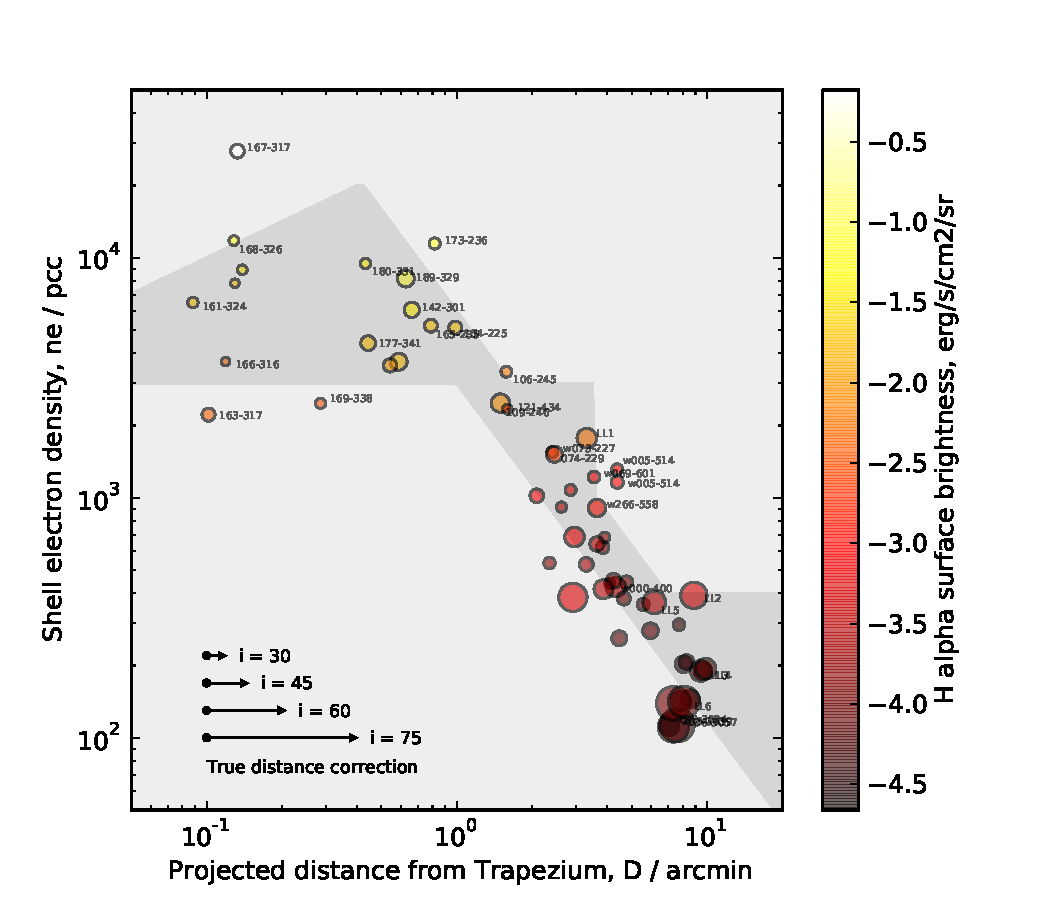
\includegraphics[width=\linewidth, clip]{luis-programas/will-nshell-vs-D.pdf}
  \caption{Densidad electrónica corregida por extinción en función de la distancia proyectada a \(\theta^1\ \text{Ori}\ \text{C}\), obtenida a partir de las observaciones de Bally, es decir usando el  brillo superficial de \(\ha\) en la cáscara chocada para determinarla. El tamaño de los puntos indica que tan grande es el camino de visión en la zona chocada si los comparamos entre si. Las flechas en la parte superior izquierda representan la distancia corregida de los arcos de emisión a \thC{}, para los ángulos de inclinación; \(i = 30^{\circ}, 45^{\circ}, 60^{\circ}, 75^{\circ}\).  Por otro lado la escala de colores representa el brillo superficial de los objetos en unidades de [\(\mathrm{erg~s^{-1}~cm^{-2}~sr^{-1}}\)]. }
  \label{fig:density}
\end{figure}

Dado que a partir de las observaciones hemos podido determinar el brillo superficial de \ha{} realizando un poco de fotometría como se puede apreciar previamente y además como tenemos el camino de la línea de visión en la cáscara chocada (\(\Delta\zeta\)), dada por la Ec. \ref{eq:vision},  hemos determinado la densidad de núcleos de Hidrógenos (\(n\))  usando la ecuación \ref{eq:densidad}, específicamente en esta región (en la cáscara) para los diferentes objetos LL y los choques de los proplyds. Hay que subrayar que hemos usado cómo distancia a la Nebulosa de Orión 436 Pc para hacer las respectivas conversiones de unidades.\\ 

En la figura \ref{fig:density} se logra apreciar que los objetos que están más cercas de las estrellas masivas del Trapecio, presentan una densidad electrónica mayor que los que se encuentran a las afueras de la nebulosa, entonces estas altas densidades electrónicas provocan que el brillo superficial, generado a partir de la emisión de la líneas de recombinación de \ha{} sea mayor en las proximidades de \thC{}. Y es que en esta región domina la emisión de \ha, es decir hay poca contaminación por las líneas de  \nii{}.\\


\subsection{Relación y diferencia entre la presión térmica en la cáscara y la presión hidrodinámica en los vientos }
\label{sec:pressure}

\begin{figure}
  \centering
  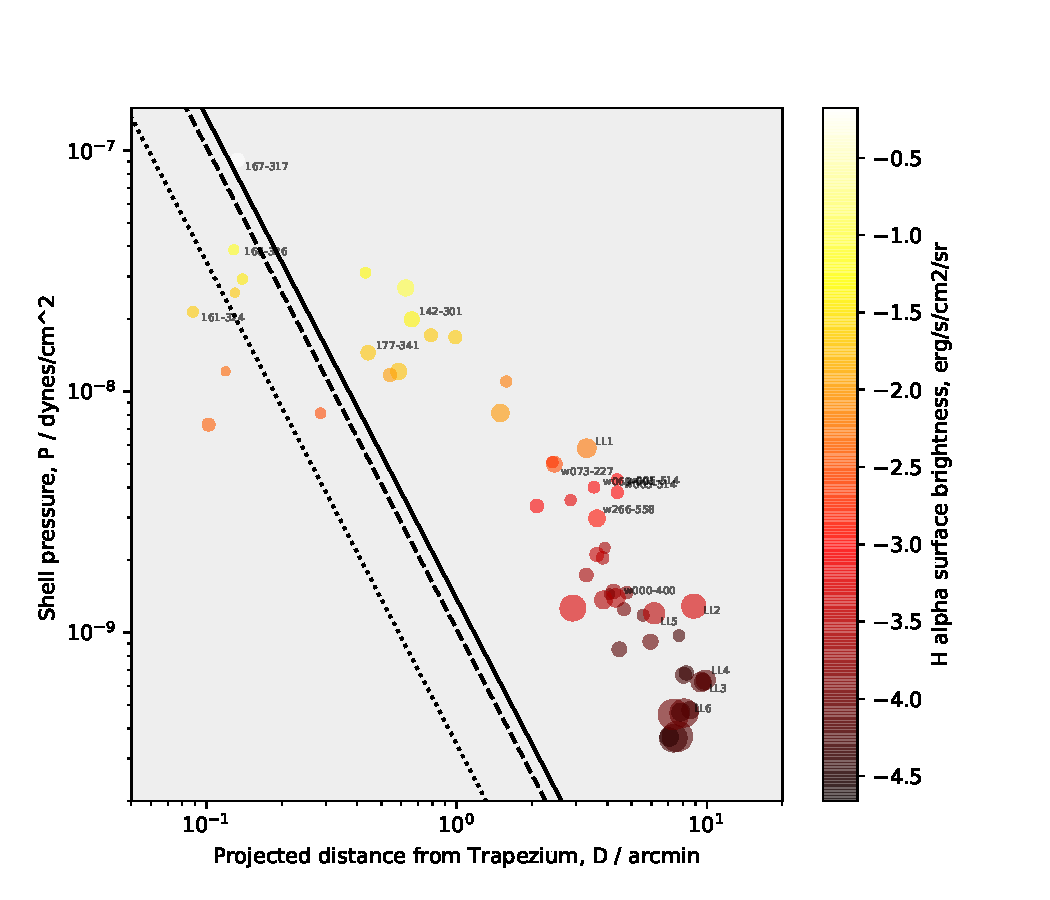
\includegraphics[width=\linewidth, clip]{luis-programas/will-Pshell-vs-D.pdf}
  \caption{Los símbolos indican la presión térmica en la cáscara chocada  y las líneas representan la presión hidrodinámica generada por el viento estelar, ambas en unidades de [\(\mathrm{dynas~cm^{-2}}\)], en función de la distancia proyectada a \thC{}. La línea continua representa la presión ram del viento estelar en función de la distancia suponiendo que no hay inclinación, esto es para \(i = 0^{\circ}\), la línea discontinua representa la misma presión ram para una distancia proyectada cuando se cambia el ángulo de inclinación desde la distancia (\(i = 0^{\circ}\)), es decir para un ángulo de inclinación de \(i = 30^{\circ}\) y la línea de puntos también representa la presión ram para una distancia proyectada con un ángulo de inclinación de \(i = 60^{\circ}\). La escala de colores indica el brillo superficial de \ha{}. }
 \label{fig:pressure}
\end{figure}

Usando la ecuación \ref{eq:presion-cascara} de \S\ref{sec:pressur-thermal} se estimó la presión térmica de la cáscara chocada, a partir de la densidad electrónica estimada en \S\ref{sec:density} y suponiendo una temperatura para esa región de \(10^{4}~\K\).\\

 Por otro lado usando la Ec. \ref{eq:presion-externa} de la misma sección determinamos la presión hidrodinámica ejercida para cada objeto por el viento estelar hipersónico de la estrella másiva \thC{} del Trapecio (usando la distancia \(D\) del objeto en cuestión a \thC{}), para una cierta tasa de pérdida de masa de \(\dot{M} = 3.5 \times 10^{-7}~\msolagno\) y una velocidad de \(v = 1200~\mathrm{km~s^{-1}}\). \\

Ahora bien, la figura \ref{fig:pressure} es el resultado de tales estimaciones. En ella estamos comparando las presiones en las cáscara chocada de los objetos LL y de los proplyds (símbolos de colores en la gráfica), con la presión ram generada por el viento estelar (lineas continuas  y discontinuas  de color  negro en la gráfica). Se observa  que la presión térmica es mayor en los objetos, que están dentro de la nebulosa,  es decir en los proplyds conocidos, a su vez esta  coincide con la presión ram del flujo de la estrella masiva, indicando que los choques de los proplyds en el interior están confinados por el hipersónico viento estelar, es posible argumentar esto considerando el equilibro de presiones (ver Ec. \ref{eq:igualda-presion}). Lo contrario sucede con los arcos hiperbólicos en las afueras de la nebulosa, puesto que la presión en la zona chocada no coincide con la presión del viento estelar, por tanto esto nos lleva a pensar que estos objetos no están interactuando con el viento estelar, sino más bien con el transónico flujo de champaña fotoevaorado proveniente del núcleo de la nebulosa.  

\subsection{Flujo de momento interno: \(\dot{M}_{w}\text{V}_{w}\) }
\label{sec:momentum}

\begin{figure}
  \centering
  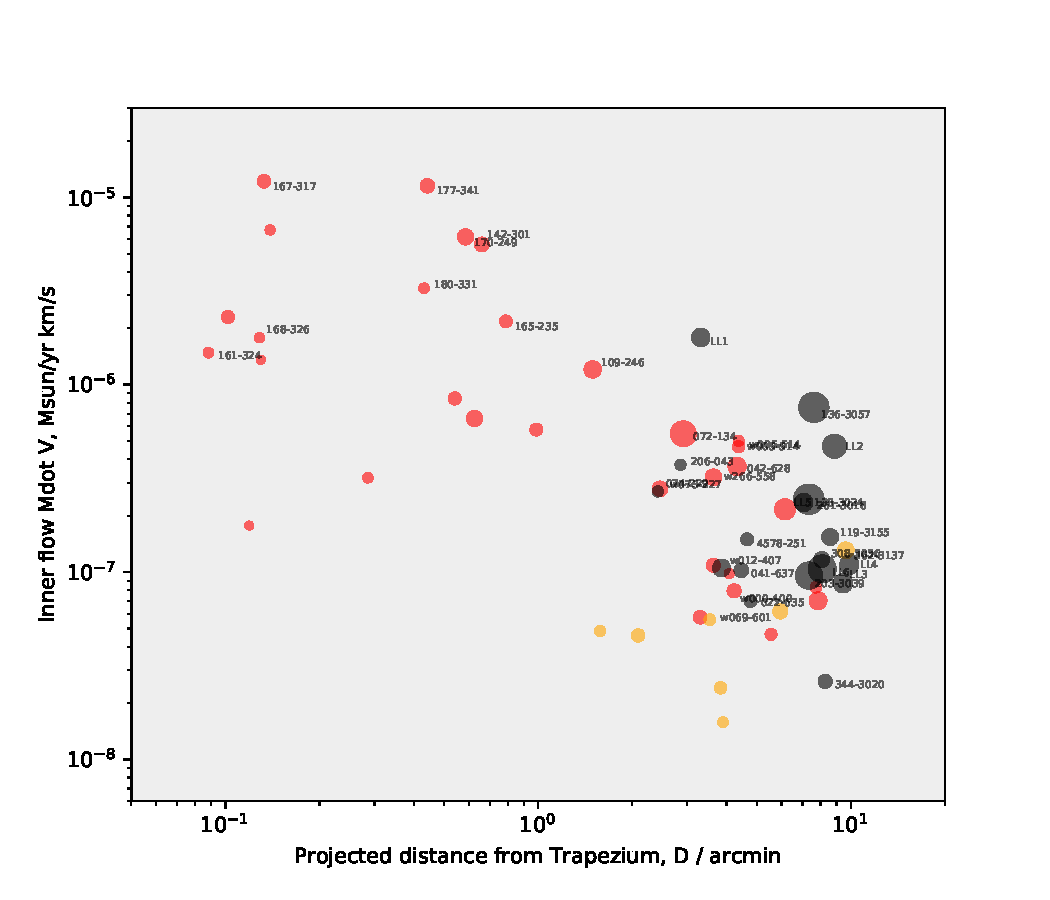
\includegraphics[width=\linewidth, clip]{luis-programas/will-MdotV-vs-D.pdf}
  \caption{Flujo de momento interno  en función de la distancia proyectada. El color de los símbolos indican: Rojo; son verdaderos proplyds, naranja; podrían tratarse de proplyds, negro; no son proplyds. El tomaño de los simbolos representan el tamaño de la línea de visión (\(\Delta\zeta\)) en la cáscara chocada.  }
 \label{fig:flow}
\end{figure}


Hemos determinado el flujo de momento interno para los objetos de nuestro catálogo a partir de las presiones de estancamiento, presiones con las cuales se obtuvo la ecuación \ref{eq:momentum}, con esta ecuación fue posible determinar el ya mencionado flujo de momento, en este orden de ideas se utilizaron los valores de la presión térmica determinados arriba, junto con los valores de los radios \(R_{0}\) internos de los choques LL para este fin. Asi que en la figura \ref{fig:flow} se ilustran dichos resultados.\\

No obstante, en la figura~\ref{fig:flow} se logra apreciar que para los objetos clasificados como proplyds en nuestro catálogo (símbolos de color rojo) y que están a cortas distancias del Trapecio presentan grandes pérdida de masa, es decir  muestran fuertes vientos, esto es debido probablemente a un incremento en el tamaño de sus discos. Ahora bien, en los proplyds y supuestos proplyds (símbolos de color naranja) ubicados en las regiones externas de la nebulosa, se observa una disminución del parámetro \(\dot{M}_{w}V_{w}\). Esto es debido a que el flujo de fotones FUV (ultravioletas lejano), responsables directo de la destrucción inevitable de los discos de acreción, decrecen con la distancia a la estrella masiva \thC{}. Por último, para el caso caso de los objetos que no son proplyds (símblos de color negro) situados en las regiones externas de la nebulosa, se observa que tienden a tener fuertes vientos. Aún no sabenos a que se debe este fenómeno.\\ 


%\bibliography{luis-ref}

%\end{document}
